\documentclass{article}
\usepackage{graphicx}
\usepackage{amsmath,cite}
\usepackage{tikz}
\usetikzlibrary{arrows}

\renewcommand{\arraystretch}{1.5}

\title{Solving small shogi}
\author{I. van Duijn \\ Utrecht University}
\begin{document}
\maketitle

\section{Abstract}
%TODO

\section{Introduction}
Ever since the early days of modern computers there has been great interest in chess programming~\cite{shannon1950xxii}. Initial
focus in the west was mainly on chess and checkers, but when computers were well established in Japan, researchers there adopted
many techniques from computer chess and applied them to their local chess variant, shogi.

\subsection{shogi}%TODO relevant citations
Shogi (Japanese chess) is a game similar to western chess. It is played on a $9 \times 9$ board and every
player has 20 pieces, some of which correspond to western pieces and others are slightly different.
Black makes the opening move and both players aim to capture the opponent's king.
The main difference between shogi and chess is the so called drop rule.
A piece that is captured by a player now belongs to him and can be placed on \textit{any} vacant square in one of his subsequent turns
(in stead moving a piece already on the board).
Additionally, in shogi nearly all pieces can promote upon moving to or from the promotion zone (starting ranks of opponent).
Unlike western chess, each type of shogi piece can only promoted to one specific piece (e.g. bishop always promotes to a dragon horse).
The drop rule, and to a lesser extent the promotion rule, dramatically increase the game tree complexity of shogi as compared to chess, see Table
\ref{table:complex} for a comparison.\\
%TODO: tabel
\begin{table}
\center
\begin{tabular}{l l l l}
 & Chess & Shogi & Go \\ \hline
State-space complexity & $10^{43}$ & $10^{71}$ & $10^{172}$ \\
Game-tree complexity & $10^{123}$ & $10^{226}$ & $10^{360}$ \\ \hline
\end{tabular}
\caption{The complexities of chess, shogi and go}
\label{table:complex}
\end{table}

Like computer chess, computer shogi is an active field of research~\cite{iida2002computer}. The main interest is how we can program computers 
such that their play peers with -- and eventually even surpasses -- human professional players. Shogi, being complexer
than western chess, has a game tree too large to make exhaustive search even near feasible. Consequently, research
focusses on clever ways to search the game tree in order to find a good heuristic. Many techniques from computer chess
have been employed, but the drop rule introduced such a novelty that new shogi-specific techniques had to be developed.\\

\subsection{Solving shogi}
Unlike in western chess, end game situations
in shogi are not significantly less complex than mid game situations. In fact, any board configuration resulting from the standard
starting setup has exactly 40 pieces in play. Because of this there is no database with solved end games for shogi.
However, in shogi, so called mating problems \footnote{On a predesigned setup, black (lacking a king) can only make checking moves},
which resemble end game situations, are extensively studied ~\cite{grimbergen1999survey}. There exist several
programs that can completely solve a lot of these problems, some of which are quite large~\cite{seo2001pn}. Unfortunately solutions to these shogi
mating problems are not the equivalent of solutions to western chess end games; in shogi, such a solution cannot be directly applied to find a winning move.
However, since the methods used to prove the shortest mating sequence are exact and not heuristical, they or similar methods might be useful to prove
certain subsets or small variants of shogi.\\

One particular method, proof-number search, has been proven to be quite effective, even outperforming $\alpha\beta$-search~\cite{van2008proof} in
proving the game theoretical value of a game tree. This method has also been succesfully applied to shogi mating
problems~\cite{seo2001pn}~\cite{ueda2008weak}~\cite{sakuta2001performance}. We will discuss the viability of using proof-number search to solve variants of shogi and will test
 this method on small shogi variants.\\

TODO: introduce all sections.

\section{Method}
We are dealing with generic small sized shogi variants, so representation and algorithms employed have to be sufficiently generic as well.
A small shogi variant is defined by the size of the board, the initial configuration of black (white's is $180^{\circ}$ rotationally symmetrical) and
the size of the promotion zone. The initial configuration consists of a set of pieces, each of which has one or two move sets (taking into account
promotion). Any algorithm that aims to prove the game theoretical value of a variant then only has to have access to two functions based on this
definition: a move generator which can map positions to a set of successing positions, and an evaluation function which recognises terminal
positions and computes their value.

\subsection{Representation}
As stated before, we have to be able to generically represent board positions. A well known technique in computer chess, bitboards, has been
shown~\cite{grimbergen2007using} to be fairly effective in shogi as well. A bitboard is a bit pattern of (at least) the size of the board,
in which each bit encodes some information (e.g. if it is occupied) about the corresponding square. Since the size of the bit pattern can
easily be increased to accomodate larger boards, they are well suited for our purpose. Also, as will be explained later, they allow for easy
generic move generation.

In the current implementation, a position is represented by one bitboard per player per piece's move set (unpromoted and promoted), plus an additional
bitboard per player containing the pieces in hand. Each bitboard corresponding to a certain piece's move set represents all pieces of that type
owned by a specific player. For an $n \times m$ board, each bitboard is fitted in the smallest $nm \leq 2^k$-bit integer (for small
variants $16$ or $32$ bit integers suffice). %TODO: example

To generate moves, we essentially need two things. We need to know for each individual piece where it is, and where it can move to in its current state.
The location of each individual piece can easily be extracted from the bitboards representing a position. To determine where it can move to, a table
is generated which maps position bitboards to move bitboards. %TODO illustrate with example

Finally, the evaluation function can use the move generator to check whether any move captures the opponent's king. Note that the evaluation function
does not give a heuristical value, it only evaluates terminal positions to nonzero values ($1$ for win and $-1$ for loss).

With the move generator and the evaluation function in place, we have an implicit definition of the game tree. The main problem of proving the game
theoretical value efficiently is only generating relevant parts of the tree.

\subsection{Proof-number Search}
Proof-number search~\cite{allis1994proof} is an algorithm designed to find the game theoretical value of a game tree, or more specifically an AND/OR tree.
The tree consists of a root, internal nodes and leaf nodes. Each node is either an AND (white to move) or an OR (black to move) node. By definition, a leaf
node represents one player's victory and thus it has a nonzero value of $1$ (black won) or $-1$ (white won). As in the minmax algorithm, an internal
node's value can be computed by taking the maximum or minimum of the children's value for AND and OR nodes respectively (Figure \ref{tree:simple}).

\begin{figure}[h]
\center
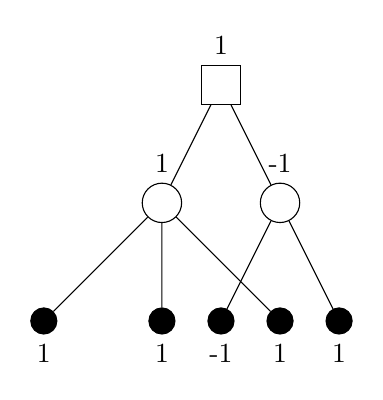
\begin{tikzpicture}[
    all/.style={minimum width=.5cm, minimum height=.5cm},
    and/.style={all, circle, draw},
    or/.style={all, rectangle, draw},
    term/.style={circle, draw=black, fill},
]
    \node [or, label=1] {} 
        child { node [and, label=1] {} 
                child { node [term, label=below:1] {} }
                child { node [term, label=below:1] {} }
                child { node [term, label=below:1] {} }
        }
        child {
            node [and, label=-1] {}
            child { node [term, label=below:-1] {} }
            child { node [term, label=below:1] {} }
        }
    ;
\end{tikzpicture}
\caption{Square AND nodes, circular OR and filled terminal nodes with their respective value.}
\label{tree:simple}
\end{figure}

The most simple form of the minmax algorithm performs a depth first traversal of the tree to calculate the value of the root. Proof-number search however
successively expands the \textit{most promising} node in the tree untill the root can be proved (i.e. determining its game theoretical value).
A node is promising if it has a small lower bound of how many other nodes need to be proved in order for it be be proved.

\subsubsection*{Most proving node}

\subsubsection*{(Dis)proof numbers}

\subsubsection*{Breadth-first search}
For comparison there is also a simple breadth-first search implementation.

\subsection{Tree vs. Graph}

\section{Result}
%subsection: Point out where and why PN fails where BFS succeeds.

%subsection: Elaborate on why PN fails on trees (splosion) and on graphs (algorithm breaks)

\section{Discussion}

\end{document}
